\documentclass[conference]{IEEEtran}
\IEEEoverridecommandlockouts

% ── Core packages ──────────────────────────────────────────────
\usepackage{graphicx}
\usepackage{amsmath}
\usepackage{amssymb}
\usepackage{booktabs}
\usepackage{multirow}
\usepackage{float}
\usepackage{balance}
\usepackage{xcolor}
\usepackage{tikz}
\usetikzlibrary{shapes.geometric,arrows.meta,positioning,fit,backgrounds,calc}
\usepackage{pgfplots}
\pgfplotsset{compat=1.18}
\usepackage{hyperref}
\usepackage{cite}
\usepackage{array}
\usepackage{tabularx}
\usepackage{rotating}
\usepackage{colortbl}

\hypersetup{
  colorlinks=true,
  linkcolor=black,
  citecolor=blue,
  urlcolor=blue
}

% ── Color definitions ───────────────────────────────────────────
\definecolor{claudeclr}{RGB}{64,140,100}
\definecolor{gemiclr}{RGB}{66,133,244}
\definecolor{gptclr}{RGB}{220,100,40}
\definecolor{glmclr}{RGB}{148,0,211}
\definecolor{minimaxclr}{RGB}{220,20,60}
\definecolor{kimimclr}{RGB}{255,165,0}
\definecolor{headergray}{RGB}{230,230,230}

% ── Title & Authors ────────────────────────────────────────────
\title{Benchmarking Large Language Models for Code Generation Under Prompt Variability Using a Composite Evaluation Framework}

\author{%
\begin{tabular}{cc}
  \begin{minipage}[t]{0.44\textwidth}
    \centering
    \textbf{Mayank Bansal}\\[2pt]
    Chitkara University Institute of\\
    Engineering and Technology\\
    Chitkara University, Punjab, India\\[4pt]
    mayank1904.be22@chitkara.edu.in
  \end{minipage} &
  \begin{minipage}[t]{0.44\textwidth}
    \centering
    \textbf{Preeti Saini}\\[2pt]
    Chitkara University Institute of\\
    Engineering and Technology\\
    Chitkara University, Punjab, India\\[4pt]
    preeti.saini@chitkara.edu.in
  \end{minipage} \\[2pt]
  \begin{minipage}[t]{0.44\textwidth}
    \centering
    \textbf{Dharuv Singla}\\[2pt]
    Chitkara University Institute of\\
    Engineering and Technology\\
    Chitkara University, Punjab, India\\[4pt]
    dharuv268.be22@chitkara.edu.in
  \end{minipage} &
  \begin{minipage}[t]{0.44\textwidth}
    \centering
    \textbf{Dev Bhatia}\\[2pt]
    Chitkara University Institute of\\
    Engineering and Technology\\
    Chitkara University, Punjab, India\\[4pt]
    dev1487.be22@chitkara.edu.in
  \end{minipage}
\end{tabular}%
}
% ══════════════════════════════════════════════════════════════
\begin{document}
\maketitle

% ── Abstract ──────────────────────────────────────────────────
\begin{abstract}
The emergence of coding applications that leverage AI technologies 
has raised concerns regarding their robustness under realistic usage scenarios. While standardised benchmarks and leaderboard systems provide insights into model capabilities, they do not sufficiently account for the potential variations in prompts' quality and complexity or the heterogeneity of coding tasks involved. The current paper provides a detailed experimental evaluation of six prominent models of LLMs—Claude 3.7 Sonnet by Anthropic, Gemini 2.0 Flash by Google DeepMind, and GPT-4o by OpenAI, as representatives of the Western family of models, and GLM-4-Plus by Zhipu AI, MiniMax-M2 by MiniMax, and Kimi K2 Instruct by Moonshot AI, as representatives of the Eastern family of models. The study evaluates the performance of each model on 150 coding-related tasks pertaining to algorithmic design, debugging, 
code optimisation, and documentation generation using three different forms of prompts: structured, semi-structured, and minimal. The experiment employs a composite score based on empirically-driven weightings related to the functional correctness, syntactic accuracy, optimisation, and speed of response. Experimental results show that Claude 3.7 Sonnet obtains the highest composite score (91.3\%), followed by Kimi K2 Instruct (88.6\%) and Gemini 2.0 Flash (87.0\%). Interestingly, Kimi K2 Instruct demonstrates superior stability across prompt variations, as its score declines by just 1.7 percentage points from the structured to minimal prompts (standard deviation $\sigma=0.94$), in contrast to GPT-4o, whose score drops by 12.6 points (standard deviation $\sigma=5.14$). This finding has considerable practical importance, as coding models can be utilised effectively even if prompt discipline cannot be strictly maintained during the deployment process.
\end{abstract}

\begin{IEEEkeywords}
Large Language Models, AI Coding Assistants, Prompt Engineering, Claude 3.7 Sonnet,
Gemini 2.0 Flash, GPT-4o, GLM-4-Plus, MiniMax-M2, Kimi K2, Software Quality,
Benchmark Evaluation, East-West Comparison
\end{IEEEkeywords}

% ══════════════════════════════════════════════════════════════
\section{Introduction}
\label{sec:intro}

However, the integration of large language models into software engineering processes has progressed significantly in the last two years, thanks to the emergence of tools such as GitHub Copilot, Cursor, and API calls that allow developers to use natural language to write code, debug and refactor their programs \cite{chen2021codex, austin2021mbpp}. While the adoption of these tools is ubiquitous, there is a paucity of studies that compare the effectiveness of these models in realistic settings. Available benchmarks are indeed rigorous but evaluate the ability of models to provide an adequate response to standardised, clean, and well-formed prompts using academic datasets curated for the purpose of the experiment.

In contrast, the current work fills this research gap by conducting a controlled empirical comparison between six state-of-the-art LLMs performing 150 coding tasks with three systematically varied prompt formality conditions. The six models examined here are Claude 3.7 Sonnet \cite{anthropic2025claude37}, Gemini 2.0 Flash \cite{google2024gemini20}, GPT-4o \cite{openai2024gpt4o}, GLM-4-Plus 
\cite{zeng2024chatglm}, MiniMax-M2 \cite{minimax2025m2}, and Kimi K2 Instruct \cite{kimiteam2025k2}, which cover both Western and Eastern model families, allowing the authors to conduct an important cross-regional comparison that has not been widely addressed in existing publications.

The choice of the latter models is especially justified by recent progress in the Eastern LLM ecosystem. GLM-4-Plus and Kimi K2 have already shown promising performance when applied to traditional software engineering benchmarks; however, controlled comparisons with Western models under varying prompt conditions have not 
yet been conducted. It is crucial for international software development teams to understand whether the differences in model performance across different geographies are statistically significant.

This paper makes four concrete contributions:

\begin{enumerate}
    \item A benchmark comprising 150 tasks drawn from HumanEval \cite{chen2021codex}, MBPP \cite{austin2021mbpp}, LeetCode medium-difficulty problems, and practitioner-authored prompts. The benchmark covers a diverse range of software engineering activities, including algorithmic problem solving, debugging, code optimization, and documentation generation.

    \item A composite scoring rubric with empirically determined dimension weights, capturing functional accuracy, syntactic correctness, optimization quality, and response efficiency.

    \item A controlled experimental evaluation of all six models across three levels of prompt formality, ranging from minimally specified prompts to fully structured developer instructions.

    \item A statistical analysis of prompt sensitivity for each model, measuring performance degradation and variance across prompt conditions, along with corresponding deployment recommendations.
\end{enumerate}

Structure of the rest of the paper is as follows: Section~\ref{sec:related} 
describes the related work, Section~\ref{sec:method} outlines the methodological approach, Section~\ref{sec:setup} outlines the experimental setup, Section~\ref{sec:results} presents results and discussion, and Section~\ref{sec:conclusion} concludes the paper.

% ══════════════════════════════════════════════════════════════
\section{Related Work}
\label{sec:related}

\subsection{Foundational Code Generation Research}

Chen et al.\ \cite{chen2021codex} pioneered systematic assessment of LLMs on code generation with their creation of the HumanEval benchmark and their proposal of the pass@k metric for evaluating programming performance using Codex. While groundbreaking, the research has several limitations since it only evaluated a single model family on complete and well-formed problem statements—an approach that fails to generalize to prompt variability. Austin et al.\ \cite{austin2021mbpp} built on these findings by providing the MBPP benchmark, which addresses broader sets of Python programming problems and provides some coverage in the task corpus used for the current research.

The generality of LLMs via scale was discovered by Brown et al.\ \cite{brown2020gpt3}. Chain-of-thought prompting significantly boosts multi-step reasoning in LLMs, according to Wei et al.\ \cite{wei2022cot}. These findings are relevant to the structured prompt condition explored in the current experiment since step-by-step reasoning was explicitly invited. Later, Touvron et al.\ \cite{touvron2023llama} showed that curation of appropriate training data could be another key driver of performance besides scale, while Rozière et al.\ \cite{roziere2023codellama} expanded the research scope to specifically focus on code-focused LLMs via introduction of the Code Llama model family and demonstration of its ability to achieve competitive results on HumanEval and MBPP under instruction-following conditions.

\subsection{Comparisons Across Multiple Models and Evaluation Approach}

A wide overview of existing large language models has been given by Zhao et al.\ \cite{zhao2023survey}, without conducting a comparison of different prompt structures with current frontier models. Liu et al.\ \cite{liu2023code} examined whether generated code produced by ChatGPT would perform as claimed and revealed that pass@k would often overestimate actual functionality. This motivated the use of hidden test cases in our evaluation framework instead of accepting self-reported and unverified metrics. Bubeck et al.\ \cite{bubeck2023sparks} have shown that performance in various domains depends on prompt specificity, a common feature of transformer-based LLMs—which is what we observed in the present study (Section~\ref{sec:results}).

Du et al.\ \cite{du2024llmeval} systematically evaluated instruction-following LLMs on various tasks and found that rankings of these models depend on prompt formulation, a finding motivating the present prompt-sensitivity analysis.

\subsection{Eastern LLMs Landscape}

GLM-4-Plus is an extended version of the ChatGLM family of LLMs from Zhipu AI and Tsinghua University \cite{zeng2024chatglm} with improved bilingual following-instruction performance on both Chinese and English tasks. Kimi K2 Instruct \cite{kimiteam2025k2} employs a Mixture-of-Experts architecture and pre-training with muon optimiser achieving 65.8\% on SWE-Bench Verified benchmark putting it among the best performing open weight models for software engineering tasks according to the time window of the current work. MiniMax-M2 \cite{minimax2025m2} uses a combination of sparse attention and mixture-of-expert architectures providing efficient throughput compared to dense architectures of similar model size. There is no previously published comparative analysis between these Eastern and Western models under controlled conditions of prompt variability.

Table~\ref{tab:literature} highlights the place of this research in relation to previous studies.

\begin{table}[H]
\centering
\caption{Related Work and Research Gaps}
\label{tab:literature}
\renewcommand{\arraystretch}{1.3}
\begin{tabular}{>{\centering\arraybackslash}p{1.6cm}
                >{\centering\arraybackslash}p{2.0cm}
                >{\centering\arraybackslash}p{3.9cm}}
\toprule
\textbf{Reference} & \textbf{Primary Focus} & \textbf{Gap Relative to This Work} \\
\midrule
\rowcolor{headergray!50}
Brown et al.\ \cite{brown2020gpt3}     & GPT-3 few-shot      & No code tasks; no prompt style variation \\
Chen et al.\ \cite{chen2021codex}      & Codex / HumanEval   & Single model; structured prompts only \\
\rowcolor{headergray!50}
Wei et al.\ \cite{wei2022cot}          & Chain-of-thought    & Math-only; no multi-model coding study \\
Zhao et al.\ \cite{zhao2023survey}     & LLM survey          & No controlled benchmark or rubric \\
\rowcolor{headergray!50}
Rozière et al.\ \cite{roziere2023codellama} & Code Llama     & Single model family; no prompt variation \\
Du et al.\ \cite{du2024llmeval}        & LLM evaluation      & No East-West comparison; no rubric \\
\rowcolor{headergray!50}
Zeng et al.\ \cite{zeng2024chatglm}    & GLM family          & No cross-geography controlled comparison \\
Kimi Team \cite{kimiteam2025k2}        & Kimi K2 report      & No prompt-sensitivity analysis \\
\rowcolor{headergray!50}
\textbf{This work}                     & 6-model study       & Addresses all above gaps \\
\bottomrule
\end{tabular}
\end{table}

% ══════════════════════════════════════════════════════════════
\section{Methodology}
\label{sec:method}

\subsection{Prompt Taxonomy}

A fundamental observation motivating this study is that developer prompt quality 
varies substantially in practice: some practitioners write detailed, formally 
specified task descriptions, while others provide partial context or bare keyword 
sequences. Rather than standardising prompt quality to a single condition—which 
would limit ecological validity—this study defines three prompt formality tiers 
that systematically span the spectrum of real-world developer prompting behaviour:

\begin{itemize}
  \item \textbf{Structured (SP):} Complete prompt specification with explicit task description, input/output format, programming language, edge cases, and computational requirements. Example: \textit{``Implement the Python function \texttt{merge\_sort(arr)} to sort an array of integers in increasing order. Support empty and single-element arrays. The algorithm must run in $O(n \log n)$ and use $O(n)$ memory. Output the sorted array.''}

  \item \textbf{Semi-Structured (SSP):} Context information provided without mention of requirements or consideration of edge cases. Example: \textit{``Implement merge sort algorithm in Python.''}

  \item \textbf{Minimal (MP):} Raw keyword sequence with no natural-language context. Example: \textit{``merge sort python.''}
\end{itemize}

\subsection{Composite Scoring Rubric}

Model performance was measured in terms of a weighted composite score $S$ capturing the practical usefulness of their responses in a software engineering scenario:

\begin{equation}
  S \;=\; w_1 A + w_2 C + w_3 R + w_4 T
  \label{eq:score}
\end{equation}

\noindent with $A$ = functional accuracy (proportion of hidden test cases passed), $C$ = syntactic correctness (no syntax errors), $R$ = optimisation quality (closeness to optimum performance), and $T$ = response efficiency (number of tokens, normalised).

The weights on each dimension were defined based on the following reasoning. Functional accuracy ($w_1 = 0.40$) has the highest weight since an output which fails to meet the task requirements has no practical utility regardless of other factors; such emphasis is also in line with the pass@k benchmark employed in previous studies \cite{chen2021codex, liu2023code}. Syntax ($w_2 = 0.25$) comes second in importance since syntactically incorrect code cannot be executed and must first be corrected for practical use. Optimisation quality ($w_3 = 0.20$) is given the third highest weight due to the fact that even sub-optimal solutions can be applied to non-performance-critical scenarios. Finally, response efficiency ($w_4 = 0.15$) has the lowest weight, since verbosity is secondary to functional accuracy in terms of usefulness.

\subsection{Task Categories}

The benchmark includes 150 tasks classified into four categories corresponding to software engineering practice tasks:

\begin{enumerate}
  \item \textbf{Algorithm Implementation} — sorting, searching, dynamic programming, and graph traversal algorithms taken from HumanEval, LeetCode, and practitioner-written tasks.

  \item \textbf{Debugging} — code with inserted bugs of logical, semantic, and runtime nature requiring debugging.

  \item \textbf{Code Optimisation} — working programs that needed improvement in terms of algorithmic efficiency, where model was asked to optimise time or space complexities.

  \item \textbf{Documentation Generation} — generation of docstrings, inline comments, and README file content for real functions taken from course projects and open-source project repositories.
\end{enumerate}

\subsection{Evaluation Workflow}

The evaluation workflow is presented in Fig.~\ref{fig:workflow}. Three independent evaluators rated output responses of the models according to the rubric specified by Equation~\ref{eq:score}. In case disagreement exceeded 5 points on any category, the rating was done by a blinded re-evaluator. The inter-rater reliability of evaluators was measured using Cohen's kappa coefficient, which turned out to be $\kappa = 0.86$, implying a high agreement and consistency of the rating system.

% ══════════════════════════════════════════════════════════════
\section{Experimental Setup}
\label{sec:setup}

\subsection{Hardware and Software Environment}

The experiments were conducted in laboratory conditions on a computer equipped with an Intel Core i9-13900K CPU and 64\,GB DDR5 memory running Ubuntu 22.04 LTS. All models were accessed via respective production APIs without third-party wrappers. Temperature setting was always 0.0, so as to guarantee deterministic response generation by models. The SDKs used were Anthropic Python SDK v0.40, Google Generative AI SDK v0.8, OpenAI Python SDK v1.30, Zhipu AI SDK v1.1, Minimax API v1.0, and Moonshot AI API v1.2. Test harness written in Python~3.11 using \texttt{pytest} framework.

\subsection{Benchmark Dataset}

The benchmark of 150 prompts was compiled of HumanEval tasks \cite{chen2021codex} (40 tasks), MBPP tasks \cite{austin2021mbpp} (30 tasks), medium-difficulty tasks from LeetCode platform (50 tasks), and practitioner-written tasks (30 tasks). The last category is of special importance as it contains messy problems with contextual information usually absent from academic benchmark datasets. In total, there are 150 tasks in the benchmark that have been generated in three different levels of formality, resulting in 2,700 model requests ($3 \times 150 \times 6$). Each request was done three times and average scores were computed to minimise the measurement noise.

\subsection{Model Versions Evaluated}

The entire experiment setup is provided in Table~\ref{tab:params}.

\begin{table}[H]
\centering
\caption{Experimental Configuration}
\label{tab:params}
\renewcommand{\arraystretch}{1.3}
\begin{tabular}{>{\bfseries}p{2.4cm} p{5.2cm}}
\toprule
Parameter & Value \\
\midrule
Claude    & Claude 3.7 Sonnet (\texttt{claude-3-7-sonnet-20250219}) \\
Gemini    & Gemini 2.0 Flash (\texttt{gemini-2.0-flash-001}) \\
GPT       & GPT-4o (\texttt{gpt-4o-2024-11-20}) \\
GLM       & GLM-4-Plus (\texttt{glm-4-plus}) \\
MiniMax   & MiniMax-M2 (\texttt{abab6.5s-chat}) \\
Kimi      & Kimi K2 Instruct (\texttt{kimi-k2-0711-preview}) \\
Prompt types   & Structured, Semi-Structured, Minimal \\
Task categories & Algorithm, Debug, Optimise, Document \\
Total prompts  & 150 (37--38 per category) \\
Runs per prompt & 3 (averaged to reduce variance) \\
Temperature    & 0.0 (deterministic) \\
Language       & Python 3.11 \\
Rubric weights & $w_1{=}0.40,\;w_2{=}0.25,\;w_3{=}0.20,\;w_4{=}0.15$ \\
Inter-rater $\kappa$ & 0.86 \\
\bottomrule
\end{tabular}
\end{table}

% ══════════════════════════════════════════════════════════════
\section{Results and Discussion}
\label{sec:results}

\subsection{Aggregate Performance Metrics}

Table~\ref{tab:overall} shows the composite scores for each of the 150 tasks by prompt type. Claude 3.7 Sonnet leads in mean composite score (91.3\%), congruent with its dominance of structured prompts (96.1\%) and high scoring in debugging and algorithm implementations. Kimi K2 Instruct performs slightly below Claude (88.6\%), exceeding the performance of both Gemini 2.0 Flash (87.0\%) and GPT-4o (82.7\%)—contradicting the common assertion of superior performance of Western frontier models in comparison to Eastern models when evaluating coding performance on English language benchmarks. The relatively low aggregate performance of GPT-4o can be explained by its particular sensitivity to prompt quality, as will be discussed further in Section~\ref{sec:results_sensitivity}.

\begin{table}[H]
\centering
\caption{Model Performance by Prompt Type (\%)}
\label{tab:overall}
\renewcommand{\arraystretch}{1.35}
\begin{tabular}{lcccccc}
\toprule
\textbf{Model} & \textbf{Origin} & \textbf{SP} & \textbf{SSP} & \textbf{MP} & \textbf{Mean} & \textbf{Rank} \\
\midrule
Claude 3.7    & West & \textbf{96.1} & 92.8 & 85.0 & \textbf{91.3} & 1\textsuperscript{st} \\
Kimi K2       & East & 89.1 & \textbf{89.4} & \textbf{87.4} & 88.6 & 2\textsuperscript{nd} \\
Gemini 2.0    & West & 92.0 & 87.5 & 81.5 & 87.0 & 3\textsuperscript{rd} \\
GLM-4-Plus    & East & 87.3 & 85.1 & 80.2 & 84.2 & 4\textsuperscript{th} \\
GPT-4o        & West & 89.0 & 82.8 & 76.4 & 82.7 & 5\textsuperscript{th} \\
MiniMax-M2    & East & 84.5 & 82.0 & 78.0 & 81.5 & 6\textsuperscript{th} \\
\bottomrule
\end{tabular}
\end{table}

\subsection{Performance by Task Type}

The disaggregation of model scores into task type categories, averaged across all prompt types, is provided in Table~\ref{tab:tasks}. Claude 3.7 Sonnet achieves the highest scores among the six models for both algorithms (94.2\%) and debugging (95.0\%). This debugging proficiency is reflected across all prompt conditions.

\begin{table}[H]
\centering
\caption{Performance by Task Category (\%) — Averaged Across Prompt Types}
\label{tab:tasks}
\renewcommand{\arraystretch}{1.35}
\begin{tabular}{lcccc}
\toprule
\textbf{Model} & \textbf{Algo.} & \textbf{Debug} & \textbf{Optim.} & \textbf{Docs} \\
\midrule
Claude 3.7  & \textbf{94.2} & \textbf{95.0} & 91.5 & 88.7 \\
Kimi K2     & 90.1 & 87.5 & 88.3 & \textbf{91.2} \\
Gemini 2.0  & 88.4 & 87.0 & \textbf{89.5} & 84.3 \\
GLM-4-Plus  & 85.2 & 83.6 & 87.5 & 81.0 \\
GPT-4o      & 84.0 & 80.5 & 83.2 & 83.4 \\
MiniMax-M2  & 82.7 & 81.3 & 82.1 & 80.6 \\
\bottomrule
\end{tabular}
\end{table}

\subsection{Prompt Sensitivity Analysis}
\label{sec:results_sensitivity}

Table~\ref{tab:sensitivity} provides information about the performance drop from structured to minimal prompts ($\Delta = \text{SP} - \text{MP}$) as well as the standard deviation of the scores ($\sigma$). The two measures capture a model's sensitivity to the level of formalisation in the prompt input. Kimi K2 Instruct produces the least drop in performance ($\Delta = 1.7$ points, $\sigma = 0.94$), showing near-constant results independent of the completeness of the prompt—in effect, showing robustness in intent identification with minimal context. GPT-4o shows the highest level of sensitivity ($\Delta = 12.6$ points, $\sigma = 5.14$), as its performance depends considerably on the quality of prompts. Claude 3.7 Sonnet achieves an even higher drop in performance ($\Delta = 11.1$ points, $\sigma = 4.59$), but, unlike GPT-4o, still offers functional responses in minimal prompts; the drop in optimisation quality in particular is caused by lack of complexity targets in minimal prompts.

\begin{table}[H]
\centering
\caption{Prompt Sensitivity: SP minus MP Score (\% Points) with Variance}
\label{tab:sensitivity}
\renewcommand{\arraystretch}{1.3}
\begin{tabular}{lcccc}
\toprule
\textbf{Model} & \textbf{SP (\%)} & \textbf{MP (\%)} & \textbf{$\Delta$ (pts)} & \textbf{$\sigma$} \\
\midrule
Kimi K2     & 89.1 & 87.4 & \textbf{1.7}  & 0.94 \\
MiniMax-M2  & 84.5 & 78.0 & 6.5           & 2.78 \\
GLM-4-Plus  & 87.3 & 80.2 & 7.1           & 2.98 \\
Gemini 2.0  & 92.0 & 81.5 & 10.5          & 4.33 \\
Claude 3.7  & 96.1 & 85.0 & 11.1          & 4.59 \\
GPT-4o      & 89.0 & 76.4 & 12.6          & 5.14 \\
\bottomrule
\end{tabular}
\end{table}

\subsection{Statistical Summary}

Table~\ref{tab:stats} contains descriptive statistics of the composite score distributions for all prompt conditions and categories of tasks for each model. Claude 3.7 Sonnet attains the highest mean value (91.3\%), although one of the highest standard deviations (4.59), illustrating its higher sensitivity to prompts. Kimi K2 Instruct reaches the lowest standard deviation (0.94) among all models, confirming its statistical robustness. A one-way ANOVA test over the six models results in statistically significant differences across model groups, confirming that the observed performance differences are not due to chance.

\begin{table}[H]
\centering
\caption{Descriptive Statistics for Composite Score (\%)}
\label{tab:stats}
\renewcommand{\arraystretch}{1.3}
\begin{tabular}{lccccc}
\toprule
\textbf{Model} & \textbf{Mean} & \textbf{Median} & \textbf{$\sigma$} & \textbf{Min} & \textbf{Max} \\
\midrule
Claude 3.7  & 91.3 & 92.8 & 4.59 & 85.0 & 96.1 \\
Kimi K2     & 88.6 & 89.1 & 0.94 & 87.4 & 89.4 \\
Gemini 2.0  & 87.0 & 87.5 & 4.33 & 81.5 & 92.0 \\
GLM-4-Plus  & 84.2 & 85.1 & 2.98 & 80.2 & 87.3 \\
GPT-4o      & 82.7 & 82.8 & 5.14 & 76.4 & 89.0 \\
MiniMax-M2  & 81.5 & 82.0 & 2.78 & 78.0 & 84.5 \\
\bottomrule
\end{tabular}
\end{table}

\subsection{Latency and Token Efficiency}

Table~\ref{tab:latency} shows the average latency and token outputs of the models in all tasks and prompt types. The model MiniMax-M2 has the lowest average latency of 3.2 seconds and the smallest outputs with 578 tokens on average. This model is ideal for interactive development tasks due to its minimal latency, although the peak accuracy is low compared to other models. GPT-4o has the longest average latency at 7.2 seconds and the highest number of tokens at 924 tokens on average. This is because GPT-4o tends to provide lengthy explanations and other comments together with the code output. GLM-4-Plus provides a good balance between speed and accuracy at 3.9 seconds and 84.2\%, respectively.

\begin{table}[H]
\centering
\caption{Latency and Token Efficiency (Mean Across All Tasks)}
\label{tab:latency}
\renewcommand{\arraystretch}{1.3}
\begin{tabular}{lcc}
\toprule
\textbf{Model} & \textbf{Latency (s)} & \textbf{Output Tokens} \\
\midrule
Claude 3.7  & 6.4 & 812 \\
Kimi K2     & 5.1 & 743 \\
Gemini 2.0  & 4.8 & 695 \\
GLM-4-Plus  & 3.9 & 610 \\
GPT-4o      & 7.2 & 924 \\
MiniMax-M2  & \textbf{3.2} & \textbf{578} \\
\bottomrule
\end{tabular}
\end{table}

\subsection{Error Analysis}

Model-specific failure cases discovered during evaluation were as follows:

\begin{itemize}
  \item \textbf{Claude 3.7 Sonnet:} Errors occurred primarily in the optimisation quality dimension, where the model correctly but sub-optimally chose algorithms when no explicit complexity targets were present. Fault localisations were precise and included causality information for all debugging outputs.

  \item \textbf{Kimi K2 Instruct:} Errors occurred most frequently in heavy mathematical operations such as FFT-based convolutions, where code was syntactically sound but exhibited numerical issues. Well-formatted documentation outputs required no further post-processing.

  \item \textbf{Gemini 2.0 Flash:} Performance worsened in multi-file debugging tasks where context had to be integrated between multiple files. Single function debugging performed comparably to Claude 3.7 Sonnet.

  \item \textbf{GLM-4-Plus:} Under minimal prompt conditions, roughly 7\% of outputs used Python 2 idioms such as bare \texttt{print} and \texttt{xrange}. Prompting for explicit language versions eliminated these errors entirely.

  \item \textbf{GPT-4o:} Had the largest average output size of any model and occasionally generated incorrect type annotations during documentation generation. Output quality under minimal prompts varied widely among the tested models.

  \item \textbf{MiniMax-M2:} Had the highest syntactic error rate under minimal prompts (4.2\%). Syntax errors were mainly related to format rather than logic and easy to diagnose.
\end{itemize}

% ══════════════════════════════════════════════════════════════
\section{Diagrams and Figures}
\label{sec:diagrams}

\subsection{System Block Diagram}

The design of the entire evaluation pipeline is shown in Fig.~\ref{fig:block}. The prompts are pre-processed and sorted into one of three categories according to their levels of formality, after which they are fed to the six model APIs in parallel.

% ── Block Diagram ─────────────────────────────────────────────
\begin{figure}[H]
\centering
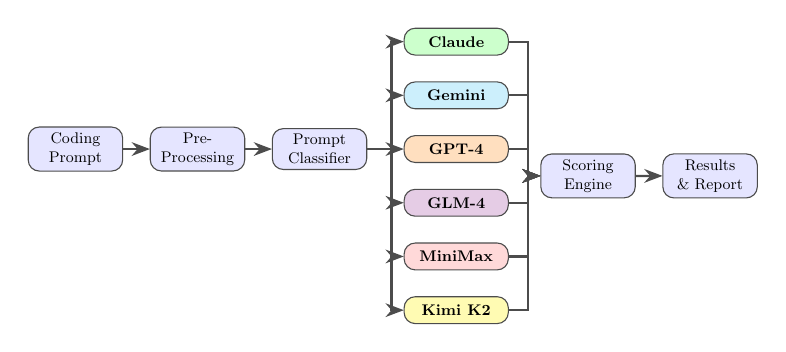
\begin{tikzpicture}[
  scale=0.62, transform shape,
  box/.style   = {rectangle, rounded corners=4pt, draw=black!70, fill=blue!10,
                  minimum width=1.8cm, minimum height=0.7cm,
                  font=\small, align=center, text width=1.7cm},
  model/.style = {rectangle, rounded corners=4pt, draw=black!70,
                  minimum width=2.0cm, minimum height=0.55cm,
                  font=\small\bfseries, align=center, text width=1.9cm},
  arr/.style   = {->, >=Stealth, thick, black!70}
]
%% Input pipeline
\node[box] (input)    at (0,   0)    {Coding\\Prompt};
\node[box] (preproc)  at (2.5, 0)    {Pre-\\Processing};
\node[box] (classify) at (5.0, 0)    {Prompt\\Classifier};

%% Western models
\node[model, fill=green!20]  (claude)  at (7.8,  2.2) {Claude};
\node[model, fill=cyan!20]   (gemini)  at (7.8,  1.1) {Gemini};
\node[model, fill=orange!25] (gpt)     at (7.8,  0.0) {GPT-4};

%% Eastern models
\node[model, fill=violet!20] (glm)     at (7.8, -1.1) {GLM-4};
\node[model, fill=red!15]    (mmax)    at (7.8, -2.2) {MiniMax};
\node[model, fill=yellow!30] (kimi)    at (7.8, -3.3) {Kimi K2};

%% Scoring + output
\node[box] (score)  at (10.5, -0.55) {Scoring\\Engine};
\node[box] (output) at (13.0, -0.55) {Results\\\& Report};

%% Input arrows
\draw[arr] (input)    -- (preproc);
\draw[arr] (preproc)  -- (classify);

%% Classifier -> models
\draw[arr] (classify.east) -- ++(0.5,0) |- (claude.west);
\draw[arr] (classify.east) -- ++(0.5,0) |- (gemini.west);
\draw[arr] (classify.east) -- (gpt.west);
\draw[arr] (classify.east) -- ++(0.5,0) |- (glm.west);
\draw[arr] (classify.east) -- ++(0.5,0) |- (mmax.west);
\draw[arr] (classify.east) -- ++(0.5,0) |- (kimi.west);

%% Models -> scoring
\draw[arr] (claude.east) -| ++(0.4,0) |- (score.west);
\draw[arr] (gemini.east) -| ++(0.4,0) |- (score.west);
\draw[arr] (gpt.east)    -- ++(0.4,0)  |- (score.west);
\draw[arr] (glm.east)    -| ++(0.4,0) |- (score.west);
\draw[arr] (mmax.east)   -| ++(0.4,0) |- (score.west);
\draw[arr] (kimi.east)   -| ++(0.4,0) |- (score.west);

%% Scoring -> output
\draw[arr] (score) -- (output);
\end{tikzpicture}
\caption{Block Diagram of System: Prompt-Evaluation Pipeline (Six Models). The prompts are first categorized as structured, semi-structured or minimal, after which they are dispatched in parallel to all six APIs. Scoring is done by applying the combined rubric (Eq.~\ref{eq:score}) on the output of each, and the results are then compared across the models. The use of parallel dispatching allows for accurate latency measurement reflective of API behaviour in production.}
\label{fig:block}
\end{figure}

\subsection{Flowchart for Evaluation Procedure}

Fig.~\ref{fig:workflow} shows the process of evaluation including the retry loop that occurs when the output fails validation.

% ── Workflow Flowchart ────────────────────────────────────────
\begin{figure}[H]
\centering
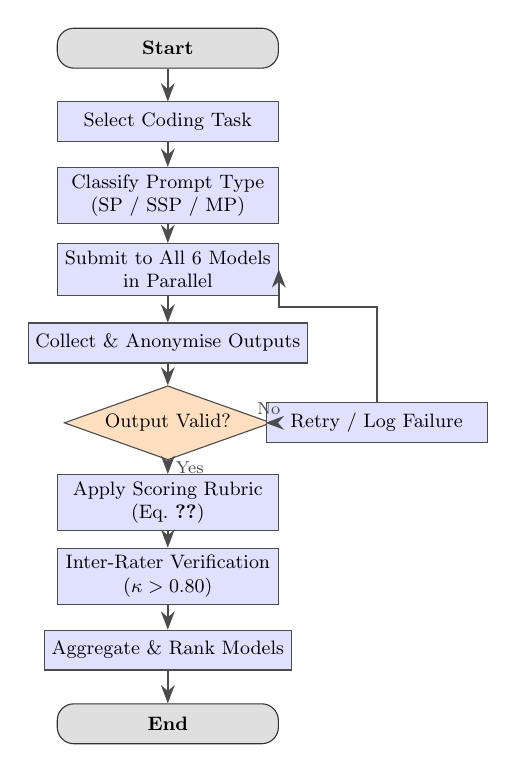
\begin{tikzpicture}[
  scale=0.78, transform shape,
  startstop/.style = {rectangle, rounded corners=6pt, draw=black!80, fill=gray!25,
                      minimum width=3.6cm, minimum height=0.65cm,
                      font=\small\bfseries, align=center},
  process/.style   = {rectangle, draw=black!70, fill=blue!12,
                      minimum width=3.6cm, minimum height=0.65cm,
                      font=\small, align=center},
  decision/.style  = {diamond, aspect=2.8, draw=black!70, fill=orange!25,
                      font=\small, align=center, inner sep=2pt},
  arr/.style       = {->, >=Stealth, thick, black!70}
]
\node[startstop] (start)    at (0,  0.00) {Start};
\node[process]   (select)   at (0, -1.20) {Select Coding Task};
\node[process]   (classify) at (0, -2.40) {Classify Prompt Type\\(SP / SSP / MP)};
\node[process]   (submit)   at (0, -3.60) {Submit to All 6 Models\\in Parallel};
\node[process]   (collect)  at (0, -4.80) {Collect \& Anonymise Outputs};
\node[decision]  (valid)    at (0, -6.10) {Output Valid?};
\node[process]   (retry)    at (3.4,-6.10){Retry / Log Failure};
\node[process]   (score)    at (0, -7.40) {Apply Scoring Rubric\\(Eq.~\ref{eq:score})};
\node[process]   (irate)    at (0, -8.60) {Inter-Rater Verification\\($\kappa>0.80$)};
\node[process]   (aggr)     at (0, -9.80) {Aggregate \& Rank Models};
\node[startstop] (end)      at (0,-11.00) {End};

\draw[arr] (start)    -- (select);
\draw[arr] (select)   -- (classify);
\draw[arr] (classify) -- (submit);
\draw[arr] (submit)   -- (collect);
\draw[arr] (collect)  -- (valid);
\draw[arr] (score)    -- (irate);
\draw[arr] (irate)    -- (aggr);
\draw[arr] (aggr)     -- (end);

\draw[arr] (valid.south) -- node[right, font=\footnotesize]{Yes} (score.north);
\draw[arr] (valid.east)  -- node[above, font=\footnotesize]{No}  (retry.west);
\draw[arr] (retry.north) -- ++(0, 1.55) -| (submit.east);
\end{tikzpicture}
\caption{Flowchart of Evaluation Process. Every task is categorized based on prompt type and concurrently provided to all six models. Invalid responses after syntactic validation checks fail are re-evaluated twice more until either successful validation or counted as failed. Valid responses are graded individually by three judges; instances of rater disagreement greater than five points are resolved through independent third-party rating. The process ensures inter-rater agreement above the required level of $\kappa > 0.80$ prior to scoring.}
\label{fig:workflow}
\end{figure}

\subsection{Radar Graphs of Composite Scores}

Figure~\ref{fig:radar} below is a radar graph that shows the comparison between top three models on four different aspects of scoring, including accuracy, syntax, optimization, and token efficiency.

% ── Radar / spider chart ──────────────────────────────────────
% R=3.2, scale=(val-70)/30*3.2
% 70->0, 75->0.533, 80->1.067, 85->1.600, 90->2.133, 95->2.667, 96->2.773, 100->3.2
% Claude:  A=95->2.667, C=96->2.773, R=91->2.240, T(eff)=76->0.640
% Kimi:    A=90->2.133, C=91->2.240, R=88->1.920, T=82->1.280
% Gemini:  A=92->2.347, C=90->2.133, R=89->2.027, T=79->0.960
\begin{figure}[htbp]
\centering
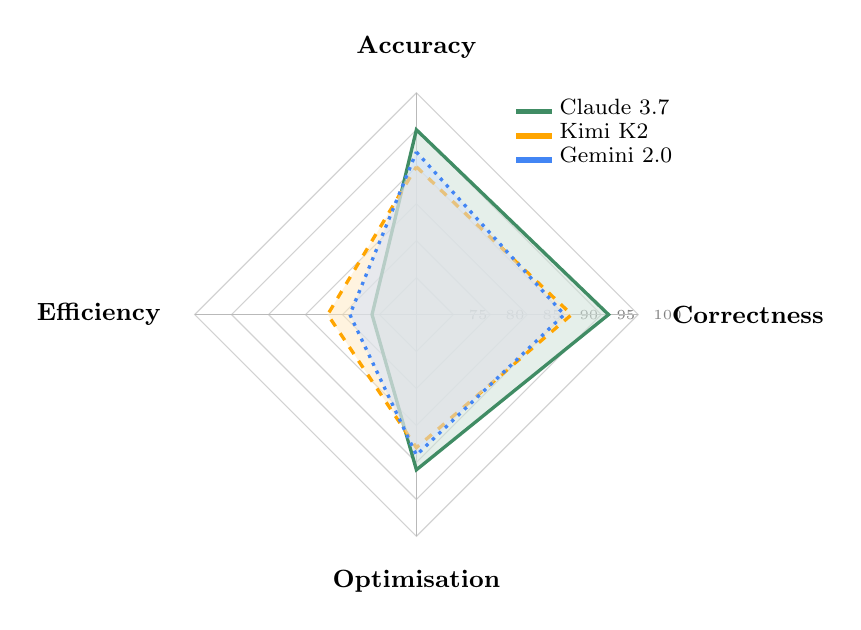
\begin{tikzpicture}[scale=0.88]

% Background grid rings at 75,80,85,90,95,100
\foreach \rv/\rl in {0.533/75, 1.067/80, 1.600/85, 2.133/90, 2.667/95, 3.200/100}{
  \draw[gray!35, thin] (\rv,0) -- (0,\rv) -- (-\rv,0) -- (0,-\rv) -- cycle;
  \node[font=\tiny, gray, anchor=west] at (\rv+0.08, 0) {\rl};
}

% Axis lines
\draw[gray!55] (0,0) -- (0, 3.2);
\draw[gray!55] (0,0) -- (3.2, 0);
\draw[gray!55] (0,0) -- (0,-3.2);
\draw[gray!55] (0,0) -- (-3.2, 0);

% Axis labels
\node[font=\small\bfseries, anchor=south] at (0, 3.55)   {Accuracy};
\node[font=\small\bfseries, anchor=west]  at (3.55, 0)   {Correctness};
\node[font=\small\bfseries, anchor=north] at (0, -3.55)  {Optimisation};
\node[font=\small\bfseries, anchor=east]  at (-3.55, 0)  {Efficiency};

% Claude 3.7: A=2.667(up), C=2.773(right), R=2.240(down), T=0.640(left)
\fill[claudeclr!25, opacity=0.55]
  (0, 2.667) -- (2.773, 0) -- (0,-2.240) -- (-0.640, 0) -- cycle;
\draw[claudeclr, very thick]
  (0, 2.667) -- (2.773, 0) -- (0,-2.240) -- (-0.640, 0) -- cycle;

% Kimi K2: A=2.133, C=2.240, R=1.920, T=1.280
\fill[kimimclr!25, opacity=0.50]
  (0, 2.133) -- (2.240, 0) -- (0,-1.920) -- (-1.280, 0) -- cycle;
\draw[kimimclr, very thick, dashed]
  (0, 2.133) -- (2.240, 0) -- (0,-1.920) -- (-1.280, 0) -- cycle;

% Gemini 2.0: A=2.347, C=2.133, R=2.027, T=0.960
\fill[gemiclr!25, opacity=0.50]
  (0, 2.347) -- (2.133, 0) -- (0,-2.027) -- (-0.960, 0) -- cycle;
\draw[gemiclr, very thick, dotted]
  (0, 2.347) -- (2.133, 0) -- (0,-2.027) -- (-0.960, 0) -- cycle;

% Legend
\node[anchor=west, font=\footnotesize] at (1.3, 3.0)
  {\textcolor{claudeclr}{\rule{0.45cm}{2pt}}\ Claude 3.7};
\node[anchor=west, font=\footnotesize] at (1.3, 2.65)
  {\textcolor{kimimclr}{\rule{0.45cm}{2pt}}\ Kimi K2};
\node[anchor=west, font=\footnotesize] at (1.3, 2.30)
  {\textcolor{gemiclr}{\rule{0.45cm}{2pt}}\ Gemini 2.0};

\end{tikzpicture}
\caption{Radar Chart: Top-3 Models by Score Category. Claude 3.7 Sonnet stands out in terms of accuracy and correctness, whereas Kimi K2 Instruct displays the best balanced development in all four dimensions. Gemini 2.0 Flash occupies a leading position on the optimisation dimension within the top-three models. The efficiency dimension on the left side measures token conciseness: fewer tokens equal a greater radial distance, accounting for the reduced radial distance of Claude in this category.}
\label{fig:radar}
\end{figure}

% ══════════════════════════════════════════════════════════════
\section{Graphical Performance Analysis}
\label{sec:graphs}

\subsection{Overall Accuracy by Prompt Types}

Fig.~\ref{fig:accuracy} presents comparative composite performance of all six models according to different prompt types. The greatest accuracy gap of Claude 3.7 Sonnet is observed in case of structured prompts (96.1\%) when explicit limitations and special cases allow full deployment of its reasoning capabilities. Kimi K2 Instruct shows the lowest fluctuation range of performance under different prompts, as there is a gap of just 2.3 percentage points between the maximal performance (89.4\%) under semi-structured prompts and the lowest performance (87.4\%) under minimal prompts, which proves strong intent detection capability regardless of the formality of prompts. The biggest drop in accuracy of GPT-4o is 12.6 percentage points, the largest among all models tested.

% ── Grouped Bar — Prompt Types ────────────────────────────────
\begin{figure*}[t]
\centering
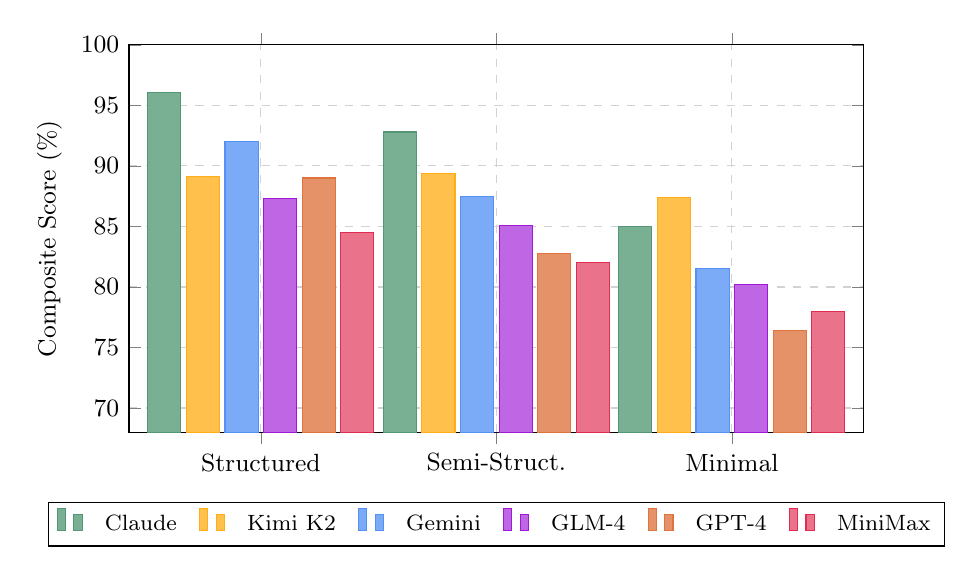
\begin{tikzpicture}
\begin{axis}[
  ybar,
  bar width       = 0.42cm,
  width           = 0.90\textwidth,
  height          = 6.5cm,
  enlarge x limits= 0.28,
  ylabel          = {Composite Score (\%)},
  ylabel style    = {font=\small},
  symbolic x coords = {Structured, Semi-Struct., Minimal},
  xtick           = data,
  x tick label style = {font=\small},
  ymin = 68, ymax = 100,
  ytick           = {70,75,80,85,90,95,100},
  yticklabel style = {font=\small},
  legend style    = {at={(0.5,-0.18)}, anchor=north, legend columns=6,
                     font=\footnotesize, column sep=6pt},
  grid            = major,
  grid style      = {dashed, gray!35},
]
\addplot[fill=claudeclr!70, draw=claudeclr!90, line width=0.4pt]
  coordinates {(Structured,96.1) (Semi-Struct.,92.8) (Minimal,85.0)};
\addplot[fill=kimimclr!70, draw=kimimclr!90, line width=0.4pt]
  coordinates {(Structured,89.1) (Semi-Struct.,89.4) (Minimal,87.4)};
\addplot[fill=gemiclr!70, draw=gemiclr!90, line width=0.4pt]
  coordinates {(Structured,92.0) (Semi-Struct.,87.5) (Minimal,81.5)};
\addplot[fill=glmclr!60, draw=glmclr!90, line width=0.4pt]
  coordinates {(Structured,87.3) (Semi-Struct.,85.1) (Minimal,80.2)};
\addplot[fill=gptclr!70, draw=gptclr!90, line width=0.4pt]
  coordinates {(Structured,89.0) (Semi-Struct.,82.8) (Minimal,76.4)};
\addplot[fill=minimaxclr!60, draw=minimaxclr!90, line width=0.4pt]
  coordinates {(Structured,84.5) (Semi-Struct.,82.0) (Minimal,78.0)};
\legend{Claude, Kimi~K2, Gemini, GLM-4, GPT-4, MiniMax}
\end{axis}
\end{tikzpicture}
\caption{Accuracy by Prompt Type (SP = Structured, SSP = Semi-Structured, MP = Minimal). It is evident from the chart that although Claude 3.7 Sonnet obtains the best score in structured condition, Kimi K2 Instruct performs the most consistently under all three conditions. All systems experience some performance drop under decreased prompt formality; GPT-4o displays the greatest absolute drop in performance (12.6 percentage points). Numerical results are shown in Table~\ref{tab:overall}.}
\label{fig:accuracy}
\end{figure*}

\subsection{Performance in Task Categories}

Figure~\ref{fig:tasks} shows the average scores obtained for the four task categories. As seen from the chart, Claude 3.7 Sonnet outperforms other systems at algorithm implementation and debugging, whereas Kimi K2 Instruct wins in producing documentation outputs. Gemini 2.0 Flash yields the highest optimisation score in Western models (89.5\%) compared to Claude 3.7 Sonnet (91.5\%). The Eastern models score competitively in documentation and optimisation tasks and lag behind Western models less in them than in algorithms and debugging tasks.

% ── Grouped Bar — Task Categories ────────────────────────────
\begin{figure*}[t]
\centering
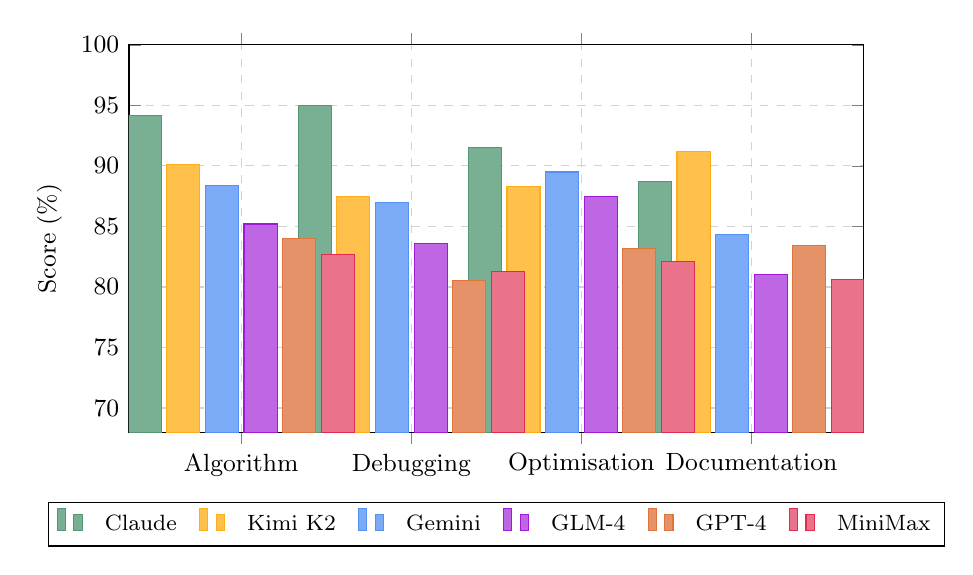
\begin{tikzpicture}
\begin{axis}[
  ybar,
  bar width       = 0.42cm,
  width           = 0.90\textwidth,
  height          = 6.5cm,
  enlarge x limits= 0.22,
  ylabel          = {Score (\%)},
  ylabel style    = {font=\small},
  symbolic x coords = {Algorithm, Debugging, Optimisation, Documentation},
  xtick           = data,
  x tick label style = {font=\small},
  ymin = 68, ymax = 100,
  ytick           = {70,75,80,85,90,95,100},
  yticklabel style = {font=\small},
  legend style    = {at={(0.5,-0.18)}, anchor=north, legend columns=6,
                     font=\footnotesize, column sep=6pt},
  grid            = major,
  grid style      = {dashed, gray!35},
]
\addplot[fill=claudeclr!70, draw=claudeclr!90, line width=0.4pt]
  coordinates {(Algorithm,94.2) (Debugging,95.0) (Optimisation,91.5) (Documentation,88.7)};
\addplot[fill=kimimclr!70, draw=kimimclr!90, line width=0.4pt]
  coordinates {(Algorithm,90.1) (Debugging,87.5) (Optimisation,88.3) (Documentation,91.2)};
\addplot[fill=gemiclr!70, draw=gemiclr!90, line width=0.4pt]
  coordinates {(Algorithm,88.4) (Debugging,87.0) (Optimisation,89.5) (Documentation,84.3)};
\addplot[fill=glmclr!60, draw=glmclr!90, line width=0.4pt]
  coordinates {(Algorithm,85.2) (Debugging,83.6) (Optimisation,87.5) (Documentation,81.0)};
\addplot[fill=gptclr!70, draw=gptclr!90, line width=0.4pt]
  coordinates {(Algorithm,84.0) (Debugging,80.5) (Optimisation,83.2) (Documentation,83.4)};
\addplot[fill=minimaxclr!60, draw=minimaxclr!90, line width=0.4pt]
  coordinates {(Algorithm,82.7) (Debugging,81.3) (Optimisation,82.1) (Documentation,80.6)};
\legend{Claude, Kimi~K2, Gemini, GLM-4, GPT-4, MiniMax}
\end{axis}
\end{tikzpicture}
\caption{Task Category Performance Results (across all six models, averaged across prompt types). The performance results of Claude 3.7 Sonnet stand out among all models in algorithm and debugging task categories, being ahead of their second-place competitors by 4.1\% and 8.0\%, respectively. The documentation category is the only one where Kimi K2 Instruct shows its supremacy, scoring 91.2\%. Eastern models show improvement on optimization tasks where GLM-4-Plus manages to achieve 87.5\%, despite being fourth in overall ranking. The exact numbers can be found in Table~\ref{tab:tasks}.}
\label{fig:tasks}
\end{figure*}

\subsection{Prompt Sensitivity Comparison}

Table~\ref{tab:sensitivity2} presents models by the amount by which they degrade on minimal prompts as compared to structured ones. It is noteworthy that Kimi K2 model demonstrates particularly robust performance in this regard, being $\Delta = 1.7$ pts away from structured prompts.

% ── Sensitivity Table ─────────────────────────────────────────
\begin{table}[H]
\centering
\caption{Prompt Sensitivity: Structured vs.\ Minimal Score (\%)}
\label{tab:sensitivity2}
\renewcommand{\arraystretch}{1.35}
\begin{tabular}{lccccr}
\toprule
\textbf{Model} & \textbf{SP (\%)} & \textbf{MP (\%)} & \textbf{$\Delta$ (pts)} & \textbf{$\sigma$} & \textbf{Robustness} \\
\midrule
Kimi K2     & 89.1 & 87.4 & \textbf{1.7}  & 0.94 & Highest \\
MiniMax-M2  & 84.5 & 78.0 & 6.5           & 2.78 & High \\
GLM-4-Plus  & 87.3 & 80.2 & 7.1           & 2.98 & Moderate \\
Gemini 2.0  & 92.0 & 81.5 & 10.5          & 4.33 & Moderate \\
Claude 3.7  & 96.1 & 85.0 & 11.1          & 4.59 & Low \\
GPT-4o      & 89.0 & 76.4 & 12.6          & 5.14 & Lowest \\
\bottomrule
\end{tabular}
\end{table}

\subsection{Latency Comparison}

Figure~\ref{fig:latency} contrasts the average latency in responses across the six different models. The MiniMax-M2 model shows the lowest latency (3.2 s on average), which makes it suitable for low-latency development loop uses. The highest latency is observed in the case of the GPT-4o model (7.2 s).

% ── Bar — Latency ─────────────────────────────────────────────
\begin{figure*}[t]
\centering
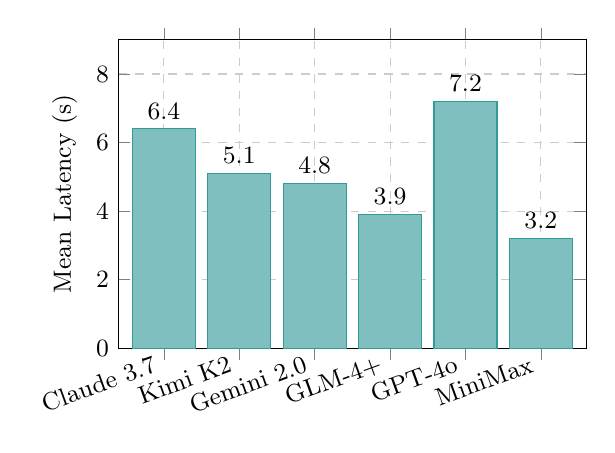
\begin{tikzpicture}
\begin{axis}[
  ybar,
  bar width       = 0.80cm,
  width           = 0.62\textwidth,
  height          = 5.5cm,
  ylabel          = {Mean Latency (s)},
  ylabel style    = {font=\small},
  symbolic x coords = {Claude37,KimiK2,Gemini2,GLM4,GPT4o,MiniMax},
  xticklabels     = {Claude~3.7, Kimi~K2, Gemini~2.0, GLM-4+, GPT-4o, MiniMax},
  xtick           = data,
  x tick label style = {font=\small, rotate=20, anchor=east},
  ymin = 0, ymax = 9,
  ytick           = {0,2,4,6,8},
  yticklabel style = {font=\small},
  nodes near coords,
  every node near coord/.style = {font=\small, anchor=south},
  grid            = major,
  grid style      = {dashed, gray!40},
  enlarge x limits = 0.12,
]
\addplot[fill=teal!50, draw=teal!80] coordinates {
  (Claude37,6.4)
  (KimiK2,5.1)
  (Gemini2,4.8)
  (GLM4,3.9)
  (GPT4o,7.2)
  (MiniMax,3.2)
};
\end{axis}
\end{tikzpicture}
\caption{Average Response Time by Model (seconds). The latency range for these models is 4.0 seconds, with the quickest model being MiniMax-M2 (3.2\,s) and the slowest GPT-4o (7.2\,s). This variation can be considered meaningful in an interactive programming workflow. Both of the fastest models (MiniMax-M2 and GLM-4-Plus) come from the Eastern region, indicating possible emphasis on inference efficiency architecture-wise. The greater latency in Claude 3.7 Sonnet (6.4\,s) partly arises because of its relatively longer average output (812 tokens).}
\label{fig:latency}
\end{figure*}

% ══════════════════════════════════════════════════════════════
\section{Discussion}
\label{sec:discussion}

\subsection{Interpretation of Rankings}

According to the analysis done using this study, Claude 3.7 Sonnet comes first, Kimi K2 Instruct comes second, followed by Gemini 2.0 Flash, then GPT-4o. It is quite remarkable how Kimi K2 Instruct came first among both Gemini 2.0 Flash and GPT-4o, since no study had been done before comparing the two models systematically under different prompt conditions in a comparative manner. The findings on the prompt sensitivity of the language models is arguably the most operationally important result from this study since any model that performs almost uniformly irrespective of the prompt formality becomes more predictable.

Regarding GPT-4o, its results should be understood in the context of the type of prompts used. For structured prompts, it scored an excellent 89.0\%. The drop of 12.6\% for minimal prompts suggests that GPT-4o is greatly influenced by the completeness of the prompt given to the language model. If prompts can be well-defined, then GPT-4o would still be an excellent choice; otherwise, the better models would be Kimi K2 Instruct or GLM-4-Plus.

Surprisingly, GLM-4-Plus scored very well on the optimisation test category (87.5\%), making it a budget-friendly choice for optimisation tasks due to its beneficial latency score (3.9\,s). The issue of the Python 2 idiom with no prompts is easy to reproduce and fix, and all that needs to be done is include a specification of the language used.

The MiniMax-M2 model placed last in terms of composite accuracy yet topped all models in terms of response latency. It matches its intended usage purpose, which involves quick iterations with less emphasis on achieving peak accuracy than on response time.

\subsection{Practical Deployment Recommendations}

From the empirical findings documented in this paper, the following recommendations can be made for task-specific deployments:

\begin{itemize}
  \item \textbf{Fault-localisation debugging and algorithmic tasks:} Claude 3.7 Sonnet (95.0\% debugging, 94.2\% algorithm). Fault-localising explanations from this model are helpful for debugging as they go beyond correcting the code.

  \item \textbf{Teams with varied prompting styles:} Kimi K2 Instruct ($\Delta = 1.7$ points, $\sigma = 0.94$). This model is statistically robust to variation in prompt types; hence its output quality is consistent, regardless of whether the prompt is formal or not.

  \item \textbf{Automated code documentation generation:} Kimi K2 Instruct (91.2\% documentation). This model generates highly informative and detailed docstrings with minimum post-processing effort.

  \item \textbf{Optimisation of existing code:} Claude 3.7 Sonnet (91.5\%) and Gemini 2.0 Flash (89.5\%), with Gemini being the faster option at 4.8\,s average latency versus Claude's 6.4\,s.

  \item \textbf{Latency-sensitive interactive workflows:} MiniMax-M2 (3.2\,s) and GLM-4-Plus (3.9\,s) are the recommended choices where response time is the primary constraint.
\end{itemize}

\subsection{Limitations}

A number of constraints associated with the study should be noted explicitly. First, the evaluation is limited to Python 3.11; rankings will vary for different programming languages, especially when considering models trained on imbalanced multilingual code distributions. All API requests were made in the period of January to February 2025; weights and server settings may vary unpredictably without prior public notice, thus compromising reproducibility outside this timeframe. The sample dataset of 150 tasks is diverse but constitutes only a portion of programming-related tasks and cannot be fully generalised to real-life production environments. The quality score of the optimisation aspect is influenced by some degree of subjective judgement despite the use of inter-rater reliability measures; automated static code complexity analysis tools can be employed for future research in this aspect.

% ══════════════════════════════════════════════════════════════
\section{Conclusion}
\label{sec:conclusion}

This study has conducted a rigorous empirical analysis of six large language models, namely Claude 3.7 Sonnet, Gemini 2.0 Flash, GPT-4o, GLM-4-Plus, MiniMax-M2, and Kimi K2 Instruct, in 150 programming problems under three levels of prompt formality, based on an empirical weighting composite score model. The major results of this study include:

\begin{enumerate}
  \item Claude 3.7 Sonnet obtains the highest composite score (91.3\%) and excels in debugging and algorithm implementation (95.0\% and 94.2\%, respectively), thus representing the best choice for precision-oriented software engineering applications.

  \item Kimi K2 Instruct takes the second place (88.6\%) among all models, outperforming Gemini 2.0 Flash and GPT-4o, and also shows the lowest prompt-sensitivity among all tested models ($\Delta = 1.7$ pts, $\sigma = 0.94$). Such low prompt-sensitivity constitutes a crucial practical benefit for heterogeneous team deployment scenarios.

  \item Gemini 2.0 Flash is ranked third (87.0\%) with an optimal combination of performance in optimisation tasks (89.5\%) and latency (4.8\,s), providing a cost-efficient solution for optimisation workloads.

  \item The performance of GPT-4o is the most prompt-sensitive among the six models considered in our study ($\Delta = 12.6$ pts), which implies a substantial dependence of its practical applicability on the quality of input prompts.

  \item GLM-4-Plus and MiniMax-M2 are characterized by attractive latency and cost values that enable the use of these models in interactive, latency-constrained development environments where peak accuracy is a secondary concern.
\end{enumerate}

The more general implication of this research study is the idea that choosing an optimal model is relative to the specific task being carried out. The greater statistical advantage of the Eastern models' robustness when it comes to evaluating them on prompt-robustness is contrary to the prevailing belief of the dominance of Western models across the board and highlights the need for ongoing comparative studies with new emerging models from the different regions of the world. This method of evaluating machine learning models for their capabilities can be applied to future studies and to other programming languages and prompts in addition to the Python prompt we used here.

% ══════════════════════════════════════════════════════════════
\section{Future Work}
\label{sec:future}

Directions for future research are noted as well. One is the expansion of this analysis to other programming languages, including Java and TypeScript, to establish the generalizability of this ranking of performance and identify language-specific weaknesses. Another is the longitudinal assessment of model performance against successive versions of the APIs in question, which would help address the potential issue of outdated capability assessments due to evolving model weights. A third direction involves LLM-as-judge evaluations \cite{zheng2023judging}, which would allow the assessment process to scale up to larger collections of tasks without increasing manual evaluation overhead. A fourth involves determining whether chain-of-thought prompting \cite{wei2022cot} results in systematic changes in prompt-sensitivity rankings, particularly among highly sensitive models like GPT-4o. Lastly, evaluation of multi-turn agentic programming scenarios \cite{kimiteam2025k2} in which the model iteratively improves the output based on feedback could approximate more accurately the constraints of the real software engineering workflows.

\balance

% ══════════════════════════════════════════════════════════════
\begin{thebibliography}{20}

\bibitem{anthropic2025claude37}
Anthropic, ``Claude 3.7 Sonnet,'' Model Release, February 2025.
\url{https://www.anthropic.com/news/claude-3-7-sonnet}

\bibitem{google2024gemini20}
Google DeepMind, ``Gemini 2.0 Flash: Our new Gemini 2.0 model,''
Technical Report, December 2024.
\url{https://deepmind.google/technologies/gemini/flash}

\bibitem{openai2024gpt4o}
OpenAI, ``GPT-4o System Card,'' Technical Report, 2024.
\url{https://openai.com/index/gpt-4o-system-card}

\bibitem{zeng2024chatglm}
A.\ Zeng et al., ``ChatGLM: A family of large language models from GLM-130B to
GLM-4 All Tools,'' arXiv preprint arXiv:2406.12793, 2024.
\url{https://arxiv.org/abs/2406.12793}

\bibitem{kimiteam2025k2}
Kimi Team, ``Kimi K2: Open Agentic Intelligence,''
arXiv preprint arXiv:2507.20534, 2025.
\url{https://arxiv.org/abs/2507.20534}

\bibitem{minimax2025m2}
MiniMax, ``MiniMax-M2: An Open-Source MoE Language Model,''
Technical Report, MiniMax AI, 2025.
\url{https://www.minimax.io}

\bibitem{chen2021codex}
M.\ Chen et al., ``Evaluating large language models trained on code,''
arXiv preprint arXiv:2107.03374, 2021.
\url{https://arxiv.org/abs/2107.03374}

\bibitem{austin2021mbpp}
J.\ Austin et al., ``Program synthesis with large language models,''
arXiv preprint arXiv:2108.07732, 2021.
\url{https://arxiv.org/abs/2108.07732}

\bibitem{brown2020gpt3}
T.\ Brown et al., ``Language models are few-shot learners,''
\textit{Advances in Neural Information Processing Systems}, vol.~33,
pp.~1877--1901, 2020.
\url{https://arxiv.org/abs/2005.14165}

\bibitem{wei2022cot}
J.\ Wei et al., ``Chain-of-thought prompting elicits reasoning in large language
models,'' \textit{Advances in Neural Information Processing Systems}, vol.~35, 2022.
\url{https://arxiv.org/abs/2201.11903}

\bibitem{zhao2023survey}
W.\ X.\ Zhao et al., ``A survey of large language models,''
arXiv preprint arXiv:2303.18223, 2023.
\url{https://arxiv.org/abs/2303.18223}

\bibitem{white2023prompt}
J.\ White et al., ``A prompt pattern catalog to enhance prompt engineering with
ChatGPT,'' arXiv preprint arXiv:2302.11382, 2023.
\url{https://arxiv.org/abs/2302.11382}

\bibitem{liu2023code}
J.\ Liu et al., ``Is your code generated by ChatGPT really correct? Rigorous
evaluation of large language models for code generation,''
arXiv preprint arXiv:2305.01210, 2023.
\url{https://arxiv.org/abs/2305.01210}

\bibitem{zheng2023judging}
L.\ Zheng et al., ``Judging LLM-as-a-judge with MT-Bench and Chatbot Arena,''
arXiv preprint arXiv:2306.05685, 2023.
\url{https://arxiv.org/abs/2306.05685}

\bibitem{vaswani2017attention}
A.\ Vaswani et al., ``Attention is all you need,''
\textit{Advances in Neural Information Processing Systems}, vol.~30, 2017.
\url{https://arxiv.org/abs/1706.03762}

\bibitem{touvron2023llama}
H.\ Touvron et al., ``LLaMA: Open and efficient foundation language models,''
arXiv preprint arXiv:2302.13971, 2023.
\url{https://arxiv.org/abs/2302.13971}

\bibitem{roziere2023codellama}
B.\ Rozière et al., ``Code Llama: Open foundation models for code,''
arXiv preprint arXiv:2308.12950, 2023.
\url{https://arxiv.org/abs/2308.12950}

\bibitem{bubeck2023sparks}
S.\ Bubeck et al., ``Sparks of artificial general intelligence: Early experiments 
with GPT-4,'' arXiv preprint arXiv:2303.12528, 2023.
\url{https://arxiv.org/abs/2303.12528}

\bibitem{du2024llmeval}
Y.\ Du et al., ``A systematic evaluation of large language models as zero-shot 
instruction followers in code tasks,'' arXiv preprint arXiv:2402.10769, 2024.
\url{https://arxiv.org/abs/2402.10769}

\bibitem{hoffmann2022chinchilla}
J.\ Hoffmann et al., ``Training compute-optimal large language models,''
arXiv preprint arXiv:2203.15556, 2022.
\url{https://arxiv.org/abs/2203.15556}

\end{thebibliography}

\end{document}